\documentclass[a4paper,10pt]{article}
%\usepackage[latin1]{inputenc} % Paquetes de idioma (otro encoding)
\usepackage[utf8]{inputenc} % Paquetes de idioma
\usepackage[spanish]{babel} % Paquetes de idioma
\usepackage{graphicx} % Paquete para ingresar gráficos
\usepackage{grffile}
\usepackage{hyperref}
\usepackage{fancybox}
\usepackage{amsmath}
\usepackage{amsfonts}
\usepackage{listings}
% Paquetes de macros de Circuitos
%\usepackage{pstricks}
\usepackage{tikz}

% Encabezado y Pié de página
\input{EncabezadoyPie.tex}
% Carátula del Trabajo
\title{ \author{} % Lo pongo para que el warning no moleste :p
\setlength{\unitlength}{1cm} %  Especifica la unidad de trabajo
\thispagestyle{empty}

\begin{picture}(18,0)
\put(0,0){\includegraphics[width=1.5cm, height=3cm]{Imagenes/Logo1.png}}

\put(10.5,0){\includegraphics[width=3cm, height=3cm]{Imagenes/Logo2.png}}

\end{picture}
\\[1.5cm]
\begin{center}
	\textbf{{\Huge Facultad de Ingenier\'ia \\ Universidad de Buenos Aires}}\\[2cm]
	{66.09 Laboratorio de Microcomputadoras}\\[0.5cm]
	{Anteproyecto}\\[2.5cm]
\end{center}

\begin{flushleft}
	\textbf{Integrantes:} \\[1cm]

	\begin{tabular}{|c|c|c|}
		\hline
		\textbf{\normalsize Padr\'on} & \textbf{\normalsize Nombre} & \textbf{\normalsize Email} \\
		\hline
		\normalsize 89579 & \normalsize Torres Feyuk, Nicol\'as R. Ezequiel & \normalsize ezequiel.torresfeyuk@gmail.com \\
		\hline
		\normalsize 90406 & \normalsize Levi Hadid, Lucas Alberto & \normalsize lucaslh9@hotmail.com \\
%		\hline
%		\normalsize ????? & \normalsize Madariaga, Eduardo & \normalsize madariagaedu@gmail.com \\
		\hline
	\end{tabular}
\end{flushleft}
\date{} % Hace que no se imprima la fecha en la cual se compilo el .tex
 }

\begin{document}
	\maketitle % Hace que el título anterior sea el principal del documento
	\newpage

	\tableofcontents % Esta línea genera un indice a partir de las secciones y subsecciones creadas en el documento
	\newpage

	\section{Proyecto: Autito RC}
		El proyecto a realizar es un autito manejado a través de comunicación inalámbrica por un medio control remoto (estos autos son los llamados \emph{RC cars}).
		Las tarea a desarrollar por el grupo consistirá en diseñar el circuito de control que permita poder manejar el autito. Para esta tarea se utilizarán dos
		microcontroladores de la familia Atmel, uno para el circuito del auto y el otro para el circuito del control remoto. \\
		\indent Además de la función básica de poder manejar al autito remota a través del control, 
		
		\indent Lalala 

	\section{Funcionalidades}
		\subsection{Control Remoto}
			\begin{itemize}
				\item Display indicador de velocidad del auto
				\item Motor erótico (te hace vibrar)
				\item Alarma de aviso de autodestrucción
				\item Medidor estado del auto
				\item Recepción de datos del auto a través del receptor (Comunicación Serie)
			\end{itemize}
		\subsection{Autito}
			\begin{itemize}
				\item Control de los Motores (mediante dos puerto H)
				\item Envío de datos de los bumpers al micro (los bumpers deben ser doble llave)
				\item Envío de datos del micro al emisor (Comunicación Serie)
			\end{itemize}

	\section{Diagramas en Bloques}
		\subsection{Autito}
			\begin{figure}[!htb]
					\centering
					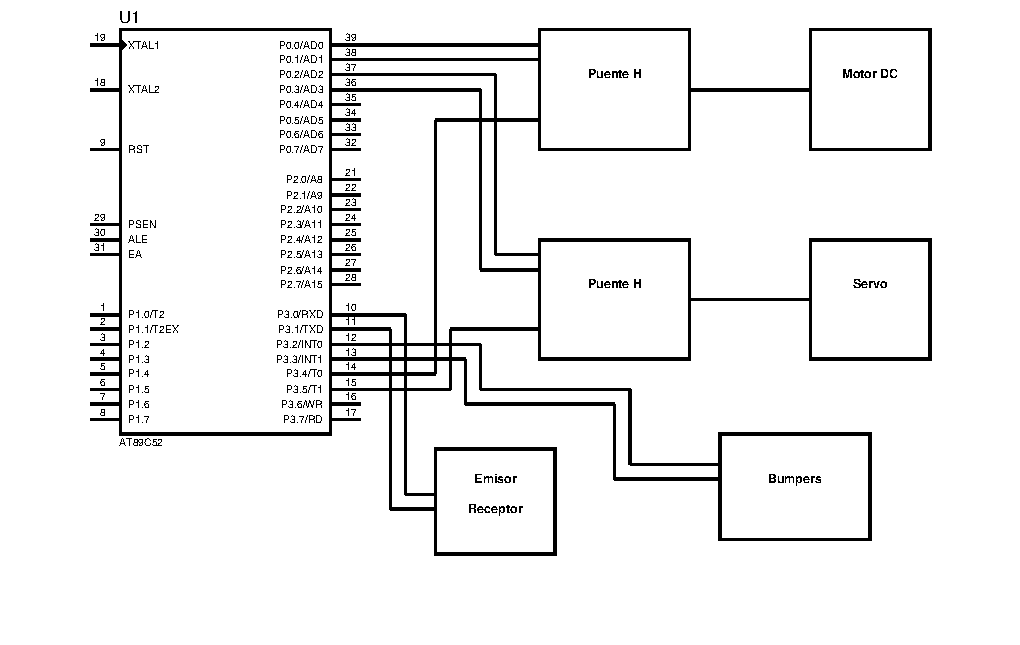
\includegraphics[width=13cm]{Imagenes/DiagramaAutito.pdf}
					\caption{Diagrama en Bloques del Autito} \label{img001}
				\end{figure}

		\subsection{Control Remoto}
		\subsection{Software}
\end{document}
